\documentclass[letterpaper,12pt]{article}
\usepackage{xcolor}
\usepackage{listings}

\definecolor{jl_background}{RGB}{253, 246, 227}
\definecolor{jl_text}{RGB}{0, 0, 0}
\definecolor{jl_comment}{RGB}{35, 129, 123}
\definecolor{jl_string}{RGB}{204, 102, 0}
\definecolor{jl_keyword}{RGB}{77, 0, 77}

\lstdefinestyle{jupyter}{
    backgroundcolor=\color{jl_background},
    basicstyle=\color{jl_text}\small\ttfamily,
    breaklines=true,
    captionpos=b,
    commentstyle=\color{jl_comment},
    keywordstyle=\color{jl_keyword},
    stringstyle=\color{jl_string},
    frame=single,
    numbers=left,
    numberstyle=\tiny\color{gray},
    showstringspaces=false,
    tabsize=4
}

\lstset{language=Python, 
    basicstyle=\ttfamily,
    keywordstyle=\color{blue}\ttfamily,
    stringstyle=\color{red}\ttfamily,
    commentstyle=\color{green}\ttfamily,
    morecomment=[l][\color{magenta}]{\#}
}

\usepackage[utf8]{inputenc} % set input encoding
\usepackage[spanish]{babel}
\usepackage{tabularx} % extra features for tabular environment
\usepackage{amsmath}  % improve math presentation
\usepackage{graphicx} % takes care of graphic including machinery
\usepackage[margin=1in,letterpaper]{geometry} % decreases margins
\usepackage{cite} % takes care of citations
\usepackage[final]{hyperref} % adds hyper links inside the generated pdf file
\hypersetup{
    colorlinks=true,       % false: boxed links; true: colored links
    linkcolor=blue,        % color of internal links
    citecolor=blue,        % color of links to bibliography
    filecolor=magenta,     % color of file links
    urlcolor=blue         
}
\usepackage{blindtext}
%++++++++++++++++++++++++++++++++++++++++


\begin{document}

\title{Solución de Sistemas de ecuaciones lineales y factorización LU con Python}
\author{Johan Posada y Juan Morales}
\date{Mayo 14 2024}
\maketitle

\section{Introducción}
La factorización LU descompone una matriz A en el producto de dos matrices: una matriz L (Lower) triangular inferior y una matriz U (Upper) triangular superior. 
Para la matriz L, todos los elementos de la diagonal son iguales a uno.
Esta factorización sigue la forma $A = L\cdot U$, solo se cumple para matrices cuadradas y es bastante usada para 
solución de sistemas de ecuaciones de la forma $Ax = b$ o para hallar el determinante: $|A| = |L|\cdot|U|$. 
El Método de reducción de Gauss-Jordan es bastante utilizado para resolver sistemas de ecuaciones de $n\cdot n$. 
El objetivo de este documento es explicar cómo se puede construir un programa en Python que permita resolver
sistemas de ecuaciones lineales de única solución y otro que haga la factorización LU de una matriz cuadrada.
\section{Construyendo el programa para Gauss-Jordan}
En un principio el programa se había construido sin usar POO, sin embargo se decidió hacer uso de este paradigma de la programación para
mejorar su estructura. El código se puede acceder en el perfil de GitHub del desarrollador del código: \url{https://github.com/johanP051/Equations-systems.git}

Para empezar, el sistema de ecuaciones lineales debe seguir esta forma:

\begin{align*}
    a_{11}x_1 + a_{12}x_2 + \cdots + a_{1n}x_n = b_1, \quad
    \\
    a_{21}x_1 + a_{22}x_2 + \cdots + a_{2n}x_n = b_2, \quad
    \\
    a_{n1}x_1 + a_{n2}x_2 + \cdots + a_{nn}x_n = b_n
    \end{align*}


\[
\left(
\begin{array}{ccc|c}
a_{11} & a_{12} & \cdots & b_1 \\
a_{21} & a_{22} & \cdots & b_2 \\
\vdots & \vdots & \ddots & \vdots \\
a_{n1} & a_{n2} & \cdots & b_n \\
\end{array}
\right)
\]
\\
Donde la última columna es el vector de igualdad. El programa se diseñó para que el usuario pueda ingresar los valores de los coeficientes y luego el de los términos
independientes, luego se encarga de realizar las operaciones necesarias para encontrar los valores de las variables o incógnitas.


Para empezar veamos el siguiente código:
\\
\begin{lstlisting}[style=jupyter, language=Python, caption={Atributos de la clase}]
    import numpy as np

    class SistemaEcuaciones:
        def __init__(self, ecuaciones, variables):
            self.ecuaciones = ecuaciones
            self.variables = variables
            
            # Lista para almacenar las filas de la matriz
            self.filas = []
            # Matriz para realizar las operaciones de Gauss-Jordan
            self.matrizReducir = None
    \end{lstlisting}

    Fíjese que se ha creado una clase llamada \textcolor{jl_keyword}{SistemaEcuaciones},
    despúes en el método \textcolor{jl_keyword}{def \_\_init\_\_} se crean los atributos del objeto: \textcolor{jl_keyword}{ecuaciones} y \textcolor{jl_keyword}{variables}
    que son los valores que se solicitarán al usuario.
    Además se crea una lista llamada \textcolor{jl_keyword}{filas} que almacenará 
    los renglones de la matriz y un arreglo llamado \textcolor{jl_keyword}{matrizReducir}
    que se usará para realizar las operaciones de Gauss-Jordan (Por el momento solo se define la variable como self.matrizReducir, por eso toma el valor \textcolor{jl_keyword}{None}, eso después va a cambiar cuando el usuario digite los datos).
    \\
    \begin{lstlisting}[style=jupyter, language=Python, caption={Método para recoger los datos}]
    def recoger_datos(self):
        for i in range(self.ecuaciones):
            elementosFila = []
            print(f"\nPara la ecuacion numero {i + 1}:")

            for j in range(self.variables):
                Xn = int(input(f"Inserte el valor del coeficiente X{j + 1}: "))
                elementosFila.extend([Xn])

            igualdad = int(input(f"A que valor esta igualada la ecuacion?: "))
            elementosFila.extend([igualdad])

            # Agregar la fila a la lista de filas, cada fila representa un solo elemento de la lista
            self.filas.append(elementosFila)
        \end{lstlisting}
Aquí se crea un método llamado \textcolor{jl_keyword}{recoger\_datos} que solicita al usuario los valores de los coeficientes de las variables y los términos independientes.
Nótese que hay un bucle for anidado, el bucle externo se usa únicamente para decirle al usuario 
cuál ecuación o fila de la matriz está digitando (i), mientras que el bucle interno se usa para recorrer las columnas (j)
solicitando los valores de los coeficientes, una vez termine este bucle se le pide el valor al que está igualada la ecuación
y el bucle externo se vuelve a repetir hasta que finalice el rango del número de ecuaciones.
Cada elemento de la fila se almacena en una lista llamada \textcolor{jl_keyword}{elementosFila} y luego cada una se agrega a la lista \textcolor{jl_keyword}{filas} que es una lista de listas.
\\

Para entender bien el siguiente método y el siguiente ejemplo sobre cómo funciona el algoritmo para reducir un sistema de 3x3, una vez se entienda, esto se puede extrapolar a una nxn.

Tomemos la siguiente matriz:
\[
\left(
\begin{array}{ccc|c}
a_{11} & a_{12} & a_{13} & b_1 \\
a_{21} & a_{22} & a_{23} & b_2 \\
a_{31} & a_{32} & a_{33} & b_3 \\
\end{array}
\right)
\]

El objetivo de la simplificacion es que los pivotes sean igual a 1. 
Si simplificamos desde la fila con índice 0 hasta la fila con índice 3, 
vamos a dividir cada fila teniendo en cuenta el elemento de la columna correspondiente, obtendremos lo siguiente:

\[
    \begin{array}{@{}cl}
    \begin{pmatrix}
        a_{11} & a_{12} & a_{13} & b_1 \\
        a_{21} & a_{22} & a_{23} & b_2 \\
        a_{31} & a_{32} & a_{33} & b_3 \\
    \end{pmatrix}
    &
    \begin{aligned}
        F_1 / a_{11} \rightarrow F_1 \\
        F_2 / a_{21} \rightarrow F_2 \\
        F_3 / a_{31} \rightarrow F_3
    \end{aligned}

    \end{array}
\]

Una vez hecho esto, se tiene una matriz simplificada que se puede reducir más fácil::

\[
    \renewcommand{\arraystretch}{2.5}
\left(
\begin{array}{ccc|c}
1 & \dfrac{a_{12}}{a_{11}} & \dfrac{a_{13}}{a_{11}} & \dfrac{b_1}{a_{11}} \\
1 & \dfrac{a_{22}}{a_{21}} & \dfrac{a_{23}}{a_{21}} & \dfrac{b_2}{a_{21}} \\
1 & \dfrac{a_{32}}{a_{31}} & \dfrac{a_{33}}{a_{31}} & \dfrac{b_3}{a_{31}} \\
\end{array}
\right)
&
\begin{aligned}
    \\
    F_2 - F_1 \rightarrow F_2 \\
    F_3 - F_1 \rightarrow F_3
\end{aligned}

\]

Reduciendo teniendo como pivote la fila 1 (indice 0):

\[
\renewcommand{\arraystretch}{2.5}
\left(
\begin{array}{ccc|c}
    1 & \dfrac{a_{12}}{a_{11}} & \dfrac{a_{13}}{a_{11}} & \dfrac{b_1}{a_{11}} \\
    0 & \dfrac{a_{22}}{a_{21}} - \dfrac{a_{12}}{a_{11}} & \dfrac{a_{23}}{a_{21}} - \dfrac{a_{13}}{a_{11}} & \dfrac{b_2}{a_{21}} - \dfrac{b_1}{a_{11}} \\
    0 & \dfrac{a_{32}}{a_{31}} - \dfrac{a_{12}}{a_{11}} & \dfrac{a_{33}}{a_{31}} - \dfrac{a_{13}}{a_{11}} & \dfrac{b_3}{a_{31}} - \dfrac{b_1}{a_{11}} \\
\end{array}
\right)

\]

\\
Ahora se debe volver a simplificar la matriz para que el pivote de la fila 2 (indice 1) sea igual a 1 y luego reducir las filas restantes.

\[
\renewcommand{\arraystretch}{3}
\left(
\begin{array}{ccc|c}
1 & \dfrac{a_{12}}{a_{11}} & \dfrac{a_{13}}{a_{11}} & \dfrac{b_1}{a_{11}} \\
0 & \dfrac{a_{22}}{a_{21}} - \dfrac{a_{12}}{a_{11}} & \dfrac{a_{23}}{a_{21}} - \dfrac{a_{13}}{a_{11}} & \dfrac{b_2}{a_{21}} - \dfrac{b_1}{a_{11}} \\
0 & \dfrac{a_{32}}{a_{31}} - \dfrac{a_{12}}{a_{11}} & \dfrac{a_{33}}{a_{31}} - \dfrac{a_{13}}{a_{11}} & \dfrac{b_3}{a_{31}} - \dfrac{b_1}{a_{11}} \\
\end{array}
\right)
&
\begin{aligned}
    \\
    \dfrac{F_2}{(a_{22}/a_{21})-(a_{12}/a_{11})} \rightarrow F_2 \\
    \dfrac{F_3}{(a_{32}/a_{31})-(a_{12}/a_{11})} \rightarrow F_3
\end{aligned}

\]

\\
La matriz simplifcada se puede reducir de nuevo teniendo como pivote la fila 2 (indice 1):

\[
\renewcommand{\arraystretch}{3.5}
\left(
\begin{array}{ccc|c}
1 & \dfrac{a_{12}}{a_{11}} & \dfrac{a_{13}}{a_{11}} & \dfrac{b_1}{a_{11}} \\
0 & 1 & \dfrac{(a_{23}/a_{21})-(a_{13}/a_{11})}{(a_{22}/a_{21})-(a_{12}/a_{11})} & \dfrac{(b_2/a_{21})-(b_1/a_{11})}{(a_{22}/a_{21})-(a_{12}/a_{11})} \\
0 & 0 & \dfrac{(a_{33}/a_{31})-(a_{13}/a_{11})}{(a_{32}/a_{31})-(a_{12}/a_{11})} & \dfrac{(b_3/a_{31})-(b_1/a_{11})}{(a_{32}/a_{31})-(a_{12}/a_{11})} \\
\end{array}
\right)
&
\begin{aligned}
    \\
    F_3 - F_2 \rightarrow F_3 \\
\end{aligned}

\]
\\

\[
    \renewcommand{\arraystretch}{3.5}
\left(
\begin{array}{ccc|c}
1 & \dfrac{a_{12}}{a_{11}} & \dfrac{a_{13}}{a_{11}} & \dfrac{b_1}{a_{11}} \\
0 & 1 & \dfrac{(a_{23}/a_{21})-(a_{13}/a_{11})}{(a_{22}/a_{21})-(a_{12}/a_{11})} & \dfrac{(b_2/a_{21})-(b_1/a_{11})}{(a_{22}/a_{21})-(a_{12}/a_{11})} \\
0 & 0 & \dfrac{(a_{33}/a_{31})-(a_{13}/a_{11})}{(a_{32}/a_{31})-(a_{12}/a_{11})} & \dfrac{(b_3/a_{31})-(b_1/a_{11})}{(a_{32}/a_{31})-(a_{12}/a_{11})}-\dfrac{(b_2/a_{21})-(b_1/a_{11})}{(a_{22}/a_{21})-(a_{12}/a_{11})} \\
\end{array}
\right)
&
\begin{aligned}
    \\
    F_3 - F_2 \rightarrow F_3 \\
\end{aligned}

\]
\\
Después se simplifica la fila 3 para lograr una matriz triangular superior con unos en la diagonal principal y ceros debajo de la diagonal principal.
De igual manera el algoritmo revisa si hay más filas restantes para reducir, en este caso no hay más filas restantes, por lo que la primera parte del proceso termina.
\\\\
Si notamos bien, el proceso se hace por cada fila y termina termina cuando las columnas de la matriz de coeficientes se acaba:
\begin{itemize}
    \item En el paso 1 se simplificó desde la fila 1 hasta la fila 3 y se redujo desde la fila 2 hasta la fila 3.
    \item En el paso 2 se simplificó desde la fila 2 hasta la fila 3 y se redujo solamente la fila 3.
    \item En el paso 3 se simplificó solamente la fila 3 y la reducción no se hace, pues en este caso la fila a reducir sería la número 4 y como no existe, entonces el bucle for no se ejecuta.
\end{itemize}
\\
\begin{lstlisting}[style=jupyter, language=Python, caption={Método para resolver el sistema de ecuaciones}]
    def gauss_jordan(self):
        inicioFilaSimplificacion = -1
        finalFilaSimplificacion = self.ecuaciones
        elementoFilaSimplificacion = -1
        
        inicioFilaReduccion = 0
        finalFilaReduccion = self.ecuaciones
        filaPivote = -1
        
        columnas = self.variables
        
        while columnas >= 1:
            inicioFilaSimplificacion += 1
            finalFS = finalFilaSimplificacion
            elementoFilaSimplificacion += 1
            #print(inicioFilaSimplificacion, finalFS, elementoFilaSimplificacion)
            # Simplificar la fila actual dividiendo por el elemento de la columna correspondiente
            for filaS in range(inicioFilaSimplificacion, finalFS):
                filaSimplificada = self.matrizReducir[filaS]
                if filaSimplificada[elementoFilaSimplificacion] != 0:
                    filaSimplificada = filaSimplificada / filaSimplificada[elementoFilaSimplificacion]
                self.matrizReducir[filaS] = filaSimplificada
        
            print(f"\nResultado de la simplificacion: ")
            print(self.matrizReducir)
        
            inicioFilaReduccion += 1
            finalFR = finalFilaReduccion
            filaPivote += 1
            #print(inicioFilaReduccion, finalFR, filaPivote)
            # Reducir las filas restantes restando la fila pivote multiplicada por el elemento correspondiente
            for filaR in range(inicioFilaReduccion, finalFR):
                filaReducida = self.matrizReducir[filaR]
                if filaReducida[filaPivote] != 0:
                    filaReducida = filaReducida - self.matrizReducir[filaPivote]
                self.matrizReducir[filaR] = filaReducida
        
            print(f"\nResultado de la Reduccion: \n{self.matrizReducir}")
        
            columnas -= 1
        print("\nSegunda parte del Gauss Jordan:")
        self.gauss_jordan_segunda_parte()

\end{lstlisting}
Como se explicó antes, en el método \textcolor{jl_keyword}{gauss\_jordan} se inicializan las variables que se usarán para simplificar y reducir la matriz mientras que el número de variables sea mayor o igual a 1.
Además, se le a agreado una condición que le indica al programa que si el elemento de la fila pivote es igual a 0, no se realice la operación de reducción.
Ni tampoco de simplificación, ya que se encontraría con una división por cero.
\\\begin{lstlisting}[style=jupyter, language=Python, caption={Método para resolver el sistema de ecuaciones}]
    def gauss_jordan_segunda_parte(self):
        inicioFilaSimplificacion = 0
        finalFilaSimplificacion = self.ecuaciones
        elementoFilaSimplificacion = self.variables

        inicioFilaReduccion = 0
        finalFilaReduccion = self.ecuaciones
        filaPivote = self.ecuaciones

        columnas = self.variables

        while columnas >= 1:
            inicioFS = inicioFilaSimplificacion
            finalFilaSimplificacion -= 1
            elementoFilaSimplificacion -= 1

            # Simplificar la fila actual dividiendo por el elemento de la columna correspondiente
            for filaS in reversed(range(inicioFS, finalFilaSimplificacion + 1)):
                filaSimplificada = self.matrizReducir[filaS]
                if filaSimplificada[elementoFilaSimplificacion] != 0:
                    filaSimplificada = filaSimplificada / filaSimplificada[elementoFilaSimplificacion]
                self.matrizReducir[filaS] = filaSimplificada

            print(f"\nResultado de la simplificacion: ")
            print(self.matrizReducir)

            inicioFR = inicioFilaReduccion
            finalFilaReduccion -= 1
            filaPivote -= 1

            # Reducir las filas restantes restando la fila pivote multiplicada por el elemento correspondiente
            for filaR in reversed(range(inicioFR, finalFilaReduccion)):
                filaReducida = self.matrizReducir[filaR]
                filaReducida = filaReducida - self.matrizReducir[filaPivote]
                self.matrizReducir[filaR] = filaReducida

            print(f"\nResultado de la Reduccion: \n{self.matrizReducir}")
            columnas -= 1
\end{lstlisting}
\\\\
En el método \textcolor{jl_keyword}{gauss\_jordan\_segunda\_parte} se realiza el mismo proceso que en el método \textcolor{jl_keyword}{gauss\_jordan} pero en sentido contrario, es decir, se simplifica y reduce desde la última fila hasta la primera.
Python en la función range() crea una lista iterable, desde la primera fila hasta la última, sin embargo, necesitamos iterar desde la última fila hasta la primera, por eso se usa la función reversed() que invierte el orden de la lista.
\\\begin{lstlisting}[style=jupyter, language=Python, caption={Método para resolver el sistema de ecuaciones}]
    # Solicitar el numero de ecuaciones y variables al usuario
    ecuaciones = int(input("Inserte el numero de ecuaciones: "))
    variables = int(input("Inserte el numero de variables: "))
    
    # Crear una instancia de la clase SistemaEcuaciones y resolver el sistema
    sistema = SistemaEcuaciones(ecuaciones, variables)
    sistema.recoger_datos()
    sistema.resolver()
\end{lstlisting}

Por último se crea el objeto sistema, haciendo una instancia a la clase \textcolor{jl_keyword}{SistemaEcuaciones} y se llama al método \textcolor{jl_keyword}{recoger\_datos} para que el usuario pueda ingresar los valores de las ecuaciones y variables.

\section*{Probando el código}
Para probar el código, se van a usar los ejercios de la página 23 del libro algebra lineal de Stanley I. Grossman, 6ta edición:
\\
\begin{minipage}{0.5\textwidth}
    \begin{align*}
        x_1 - 2x_2 + 3x_3 &= 11 \\
        4x_1 + x_2 - x_3 &= 4 \\
        2x_1 - x_2 + 3x_3 &= 10
    \end{align*}
    \end{minipage}
    \begin{minipage}{0.5\textwidth}
    \begin{align*}
        -2x_1 + x_2 + 6x_3 &= 18 \\
        5x_1 + 0x_2 + 8x_3 &= -16 \\
        3x_1 + 2x_2 - 10x_3 &= -3
    \end{align*}
    \end{minipage}

\begin{figure}[htbp]
    \centering
    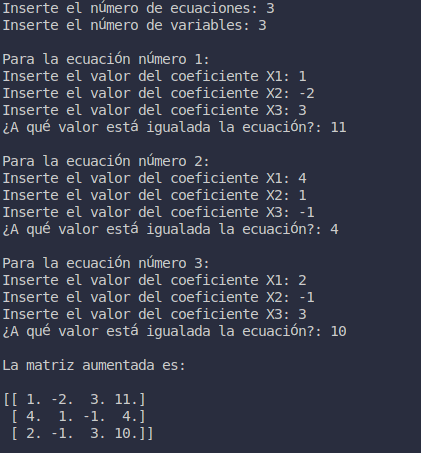
\includegraphics[width=0.9\textwidth]{/media/sebas/Exdrive/Equations-systems/imagenes/ejecucion1_0.png}
    \caption{Solicitando datos y construyendo la matriz aumentada}
    \label{fig: Matriz aumentada ejemplo 1}
\end{figure}

\begin{figure}[htbp]
    \centering
    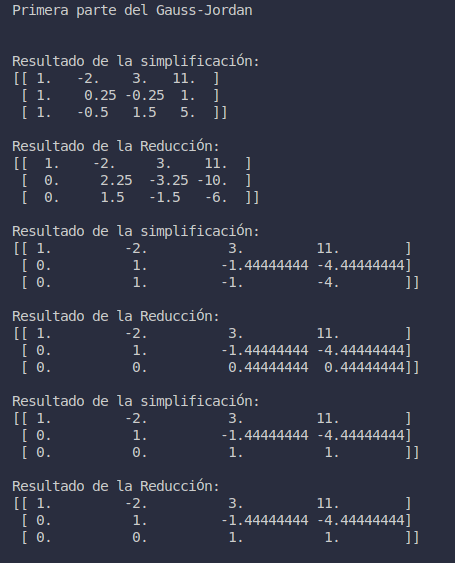
\includegraphics[width=0.9\textwidth]{/media/sebas/Exdrive/Equations-systems/imagenes/ejecucion1_1.png}
    \caption{Gauss-Jordan primera parte ejemplo 1}
    \label{fig: Gauss-Jordan primera parte ejemplo 1}
\end{figure}

\begin{figure}[htbp]
    \centering
    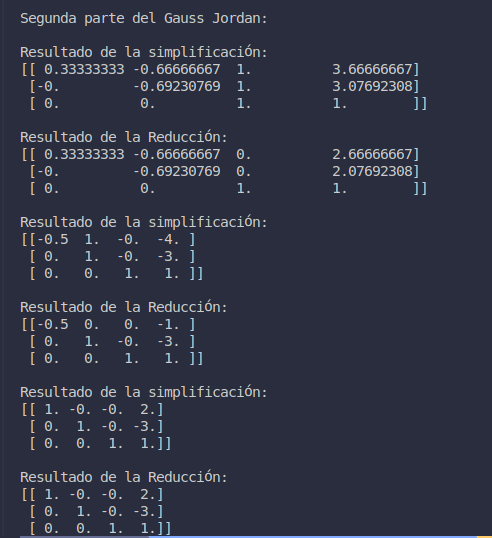
\includegraphics[width=0.9\textwidth]{/media/sebas/Exdrive/Equations-systems/imagenes/ejecucion1_2.png}
    \caption{Gauss-Jordan segunda parte ejemplo 1}
    \label{fig: Gauss-Jordan segunda parte ejemplo 1}
\end{figure}

\begin{figure}[htbp]
    \centering
    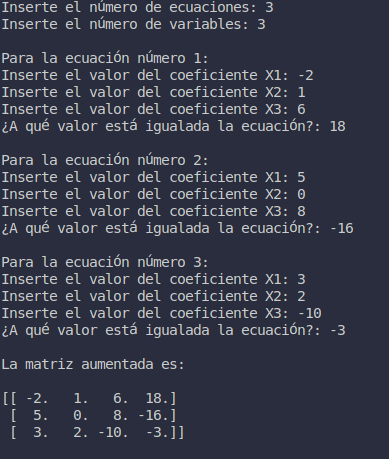
\includegraphics[width=0.9\textwidth]{/media/sebas/Exdrive/Equations-systems/imagenes/ejecucion2_0.png}
    \caption{Solicitando datos y construyendo la matriz aumentada ejemplo 2}
    \label{fig: Matriz aumentada ejemplo 2}
\end{figure}

\begin{figure}[htbp]
    \centering
    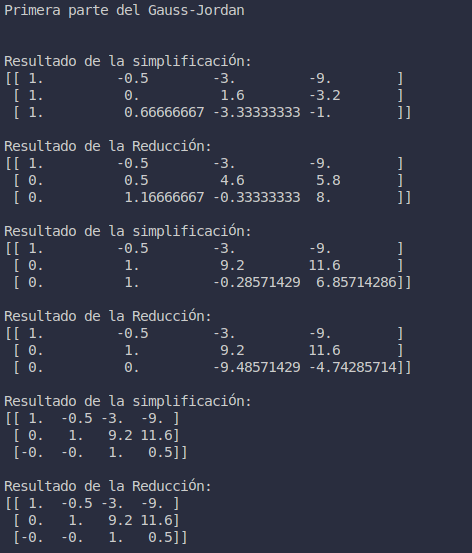
\includegraphics[width=0.9\textwidth]{/media/sebas/Exdrive/Equations-systems/imagenes/ejecucion2_1.png}
    \caption{Gauss-Jordan primera parte ejemplo 2}
    \label{fig: Gauss-Jordan primera parte ejemplo 2}
\end{figure}

\begin{figure}[htbp]
    \centering
    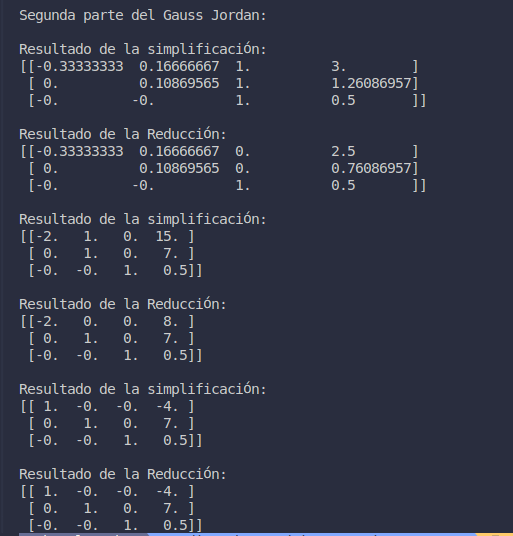
\includegraphics[width=0.9\textwidth]{/media/sebas/Exdrive/Equations-systems/imagenes/ejecucion2_2.png}
    \caption{Gauss-Jordan segunda parte ejemplo 2}
    \label{fig: Gauss-Jordan segunda parte ejemplo 2}
\end{figure}

\section*{Construyendo el programa para Factorización LU}

Antes de ver el código vamos a ver un ejemplo para una matriz 3x3:
\\
Primero se debe reducir la matriz A a una matriz triangular superior U, para esto, los elementos debajo de la diagonal principal se reducen hasta que sean iguales a 0.
Cada factor de multiplicación que se use para reducir las filas debe ponerse en la matriz L, esta es igual a la matriz identidad, con la excepcion de que debajo de la diagonal principal se encuentran los factores de multiplicación.
\[
U =
\renewcommand{\arraystretch}{1.7} 
\left(
\begin{array}{ccc}
a_{11} & a_{12} & a_{13} \\
a_{21} & a_{22} & a_{23} \\
a_{31} & a_{32} & a_{33} \\
\end{array}
\right)
&
\begin{aligned}
    \\
    F_2 - \dfrac{a_{21}}{a_{11}}\cdot F_1 \rightarrow F_2 \\
    F_3 - \dfrac{a_{31}}{a_{11}}\cdot F_1 \rightarrow F_3
\end{aligned}

\]

\[
U = 
\renewcommand{\arraystretch}{2.5}
\left(
\begin{array}{ccc}
a_{11} & a_{12} & a_{13} \\
0 & a_{22}-\dfrac{a_{21}}{a_{11}}\cdot a_{12} & a_{23}-\dfrac{a_{21}}{a_{11}}\cdot a_{13} \\
0 & a_{32}-\dfrac{a_{31}}{a_{11}}\cdot a_{12} & a_{33}-\dfrac{a_{31}}{a_{11}}\cdot a_{13} \\
\end{array}
\right)
&
\begin{aligned}
    F_3 - \dfrac{a_{32}-(a_{31}/a_{11})\cdot a_{12}}{a_{22}-(a_{21}/a_{11})\cdot a_{12}}\cdot F_2 \rightarrow F_3
\end{aligned}
\]

\[
U = 
\renewcommand{\arraystretch}{2.5}
\left(
\begin{array}{ccc}
a_{11} & a_{12} & a_{13} \\
0 & a_{22}-\dfrac{a_{21}}{a_{11}}\cdot a_{12} & a_{23}-\dfrac{a_{21}}{a_{11}}\cdot a_{13} \\
0 & 0 & (a_{33}-\dfrac{a_{31}}{a_{11}}\cdot a_{13})-(\dfrac{a_{32}-(a_{31}/a_{11})\cdot a_{12}}{a_{22}-(a_{21}/a_{11})\cdot a_{12}})\cdot (a_{23}-\dfrac{a_{21}}{a_{11}}\cdot a_{13})\\
\end{array}
\right)
\]
\\
Una vez se tiene la matriz U, se puede hallar la matriz L, reemplazando los factores de multiplicación en las posiciones L[2, 1], L[3, 1] y L[3, 2].
\\\\

\[
L =
\renewcommand{\arraystretch}{2.5} 
\left(
\begin{array}{ccc}
1 & 0 & 0 \\
\dfrac{a_{21}}{a_{11}} & 1 & 0 \\
\dfrac{a_{31}}{a_{11}} & \dfrac{a_{32}-(a_{31}/a_{11})\cdot a_{12}}{a_{22}-(a_{21}/a_{11})\cdot a_{12}} & 1 \\
\end{array}
\right)
\]
\\
Estas conclusiones se pueden extrapolar a una matriz $n\cdot n$.
\\

\begin{lstlisting}[style=jupyter, language=Python, caption={Construyendo la Matriz A}]
    import numpy as np

    dim_A = int(input("Ingrese la dimension de la matriz cuadrada A: "))
    A = np.zeros((dim_A, dim_A))
    
    for i in range(dim_A):
        for j in range(dim_A):
            A[i, j] = float(input(f"Ingrese el elemento A[{i + 1}, {j + 1}]: "))
\end{lstlisting}
\\
Aquí se solicita al usuario que ingrese la dimensión de la matriz cuadrada y luego los elementos de la matriz A, 

para esto se usa un bucle for anidado que recorre las filas (i) y columnas (j) de la matriz.
\\
\begin{lstlisting}[style=jupyter, language=Python, caption={Factorizando}]
    # Factorizacion LU
    L = np.identity(dim_A)
    U = A.copy()
    
    for j in range(dim_A):
        for i in range(j+1, dim_A):
            # Factor que multiplica a la fila j para igualarlo al elemento [i, j] de la matriz U y que al restarlos de 0
            factor = U[i, j] / U[j, j]
    
            # Se actualiza la matriz L con el factor
            L[i, j] = factor
            # Se reduce la fila i de la matriz U
            U[i] = U[i] - factor * U[j]
    
    print(f"Matriz A: \n{A}\n Matriz L: \n{L}\n Matriz U: \n{U}\n")
    
    print("Verificacion: L * U = A")
    print(np.dot(L, U))
\end{lstlisting}

\begin{itemize}
    \item Empezamos difiniendo a L como una matriz identidad, para posteriormente poder modifcarla con los factores de multiplicación.
    \item Luego se define a U como una copia de la matriz A, pues necesitamos aplicar una reducción de Gauss para hallar U.
    \item Vamos a decir que los pivotes siempre se van a encontrar en la diagonal de la matriz U, van a cambiar conforme se cambie de columna, por ejemplo, para reducir las filas de la columna 1, el pivote es U[1][1], para la columna 2, el pivote se encuentra es U[2][2], por lo que podemos decir que los pivotes son U[j][j].
    \item Por cada columna [j] se reducen las filas que están debajo del pivote, o dicho de otra manera filas con índice j + 1, por ejemplo, para el pivote U[2][2], se reducen las filas 3 (2+1) hasta n. Si a la fila [i] le asignamos el valor que tiene y le restamos el factor multiplicado por la fila en la que se encuentra el pivote, entonces la fila [i] se va a reducir.
    \item Como se pudo dar cuenta anteriormente en el ejemplo dado, por cada columna se deben recorrer las filas, por eso el bucle externo recorre las columnas [j] y el interno las filas [i].
\end{itemize}

\section*{Probando el código}
Para probar el código se va a usar la página 135 del libro algebra lineal de Stanley I. Grossman, 6ta edición:

\begin{align*}
    \begin{pmatrix}
        -1 & 2 & 3 \\
        2 & 1 & 7 \\
        1 & 3 & 10
    \end{pmatrix}
    \quad
    \begin{pmatrix}
        2 & 3 & 2 & 4 \\
        4 & 10 & -4 & 0 \\
        -3 & -2 & -5 & -2 \\
        -2 & 4 & 4 & -7
    \end{pmatrix}
\end{align*}

\begin{figure}[htbp]
    \centering
    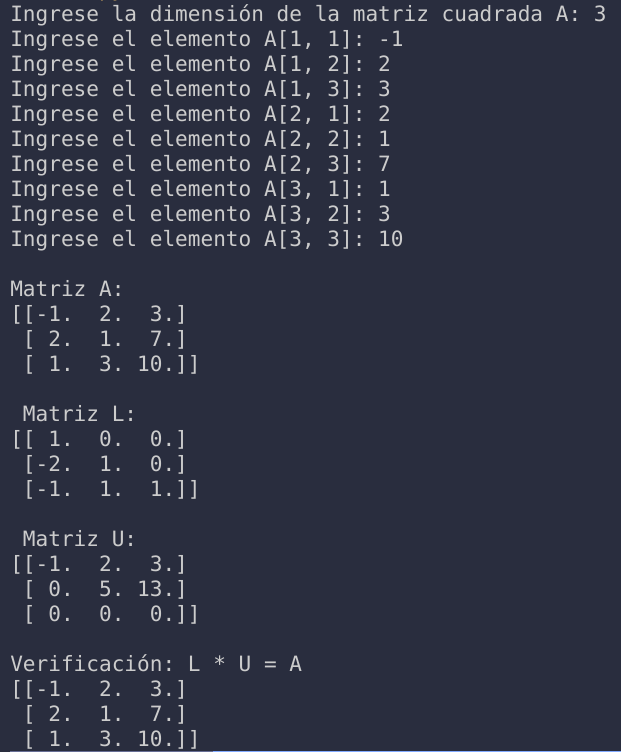
\includegraphics[width=0.4\textwidth]{/media/sebas/Exdrive/Equations-systems/imagenes/LU1_1.png}
    \caption{Factorización LU segundo ejemplo}
    \label{fig: Factorización LU segundo ejemplo}
\end{figure}

\begin{figure}[htbp]
    \centering
    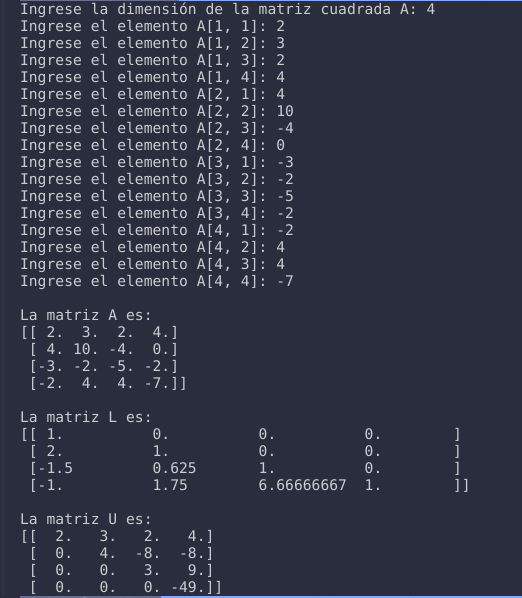
\includegraphics[width=0.7\textwidth]{/media/sebas/Exdrive/Equations-systems/imagenes/LU1_0.png}
    \caption{Factorización LU primer ejemplo}
    \label{fig: Factorización LU segundo ejemplo}
\end{figure}

\section{Conclusión}

\begin{itemize}
    \item En este documento se explicó de manera detallada el algoritmo de Gauss-Jordan, para la factorización LU se intentó usar este mismo, sin embargo el código era bastante extenso, por lo que se construyó desde cero.
    \item Cuando desarrollamos el programa para la factorización LU ya teníamos más conocimiento sobre el funcionamiento de los arreglos, por lo que fue más fácil de construir y se emplearon menos líneas de código para la reducción de Gauss.
    \item Para mejorar el programa se podría reducir la cantidad de lineas de código y no realizar tantas simplificaciones, pues se puede perder exactitud al realizar divisiones con tipos de datos de punto flotante.
\end{itemize}
\\
\begin{thebibliography}{99}
\bibitem{torres_solis}
Torres Solís, M., Villalobos Castillo, N. (s.f). Factorización LU. Universidad del Bío-Bío. Recuperado de \url{http://repobib.ubiobio.cl/jspui/bitstream/123456789/1811/1/Torres_Solis_Marcos.pdf}

\end{thebibliography}
\end{document}
